\documentclass[journal,12pt,twocolumn]{article}
\usepackage{graphicx}
\usepackage[none]{hyphenat}
\usepackage[margin=0.5in]{geometry}
\usepackage[cmex10]{amsmath}
\usepackage{array}
\usepackage{booktabs}
\usepackage{gensymb}
\usepackage{textcomp}
\title{\textbf{Line Assignment}}
\author{Dulla Srinivas - FWC22041}
\date{\today}
\providecommand{\norm}[1]{\left\lVert#1\right\rVert}
\providecommand{\abs}[1]{\left\vert#1\right\vert}
\let\vec\mathbf
\newcommand{\myvec}[1]{\ensuremath{\begin{pmatrix}#1\end{pmatrix}}}
\newcommand{\mydet}[1]{\ensuremath{\begin{vmatrix}#1\end{vmatrix}}}
\providecommand{\brak}[1]{\ensuremath{\left(#1\right)}}

\begin{document}

\maketitle
\section*{Problem Statement:}
\paragraph{The straight line 5x +4y = 0 passes through the point of
intersection of the straight lines x + 2y - 10 =0 and
2x+y+5=0. Find the point of intersection of 2 and 3 lines . and then passes 1st eqaution in 3rd equation.}

\section*{Solution:}

\begin{figure}[h]
\centering
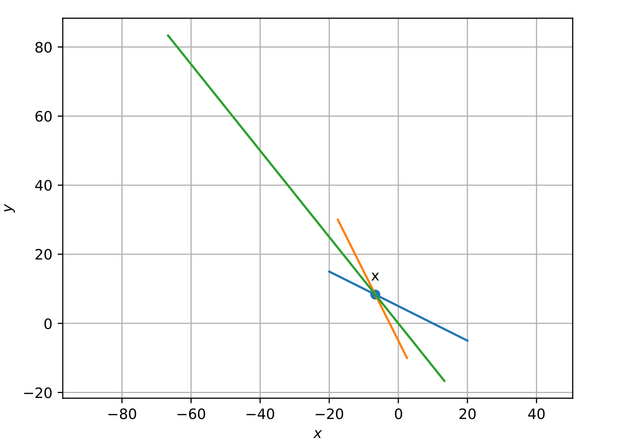
\includegraphics[width=\columnwidth]{rsz_line.png}
\caption{Diagram generated using python}
\label{fig:square}
\end{figure}
\subsection{Theory:}
They given three lines one line i.e) 5x + 4y =0 passes through the point of
intersection of the straight lines x + 2y - 10 =0 and
2x+y+5=0.}

\subsection{Mathematical Calculation:}
$\vec{O} = \myvec{0\\0}$ 
\end{center}
Given line equations are
\begin{equation}
x + 2y =10  
\end{equation}
\begin{equation}
2x+y =-5
\end{equation}

The vector equation of the line x+2y-10=0 is
\begin{eqnarray}
 (1\;2)\myvec{x\\y-5}=0
\end{eqnarray}
The vector equation of the line 2x+y+5=0  is
\begin{eqnarray}
  (7\;-1)\myvec{x\\y+5}=0
\end{eqnarray}
The point of intersection of  eq(3) and eq(4) is

\end{equation}
The vector equation of the line 5x+4y=0 is
\begin{eqnarray}
 (5\;4)\myvec{x\\y}=0
\end{eqnarray}
by passing  C in  eq(6)   5x+4y=0 we get 0
\begin{equation}
 \vec{C2} = \myvec{-100/3\\100/3}
\label{eq4}
\end{equation}
\end{equation}

Hence 5x+4y=0 passes through the point of intersection 0f 1 and 2

\section{Construction:}
The construction of given lines can be done only the x and y of given equations
\begin{table}[h]
\centering
\setlength\extrarowheight{2pt}
 \begin{tabular}{|c|c|c|}
  \hline
  \textbf{variable} & \textbf{point} & \textbf{Description}\\
  \hline
  X & (x/y) & point of intersection \\
  \hline
  Y & (x1/y1) & point of intersection \\
  \hline
  line1 & x+2y=10 & -6,8\\
  \hline                   
  line2 & 2x+y=-5 & -6,8\\
  \hline
  line3 & 5x+y=0 & -6,8\\
  \hline
 \end{tabular}
\end{table}

\end{document}